\documentclass{IEEEcsmag}

\usepackage[colorlinks,urlcolor=blue,linkcolor=blue,citecolor=blue]{hyperref}

\usepackage{tabularx}
\usepackage{upmath}
\usepackage{amssymb}
\usepackage{amsmath}
\usepackage{array}
\usepackage{arydshln}
\usepackage{listings, multicol}
\usepackage{filecontents}
\usepackage{parcolumns}


\newcolumntype{P}[1]{>{\centering\arraybackslash}p{#1}}

\jvol{XX}
\jnum{XX}
\paper{8}
\jmonth{May/June}
\jname{Computing in Science and Engineering}
\pubyear{2021}
\newtheorem{theorem}{Theorem}
\newtheorem{lemma}{Lemma}

\setcounter{secnumdepth}{0}

\lstset{language=Python, basicstyle=\ttfamily\footnotesize}

\begin{filecontents*}{loop_fusion.py}
import numba
import numpy as np

# optionally the decorator can take
# the option nopython=True, which
# disallows Numba from running in
# object mode
@numba.jit
def loop_fusion(a):
    """
    An example of loop fusion, an
    optimization that Numba is able
    to perform on a user's behalf.
    When it recognizes that they are
    operating similarly on a single
    data structure
    """
    for i in range(10):
        a[i] += 1

    for i in range(10):
        a[i] *= 5

    return a
\end{filecontents*}

\begin{filecontents*}{nested_function.py}
import numpy as np
import numba
import numba.core
import numba.typed


# Dictionary instance created at runtime
results = numba.typed.Dict.empty(
    key_type=numba.core.types.unicode_type,
    value_type=numba.core.types.float64[:]
)

@numba.njit
def nested(input, results):
    # This function expects a
    # typed dictionary as an
    # argument to store results

    def step1(a):
        # first step of algorithm
        # store results in dictionary
        ...

    def step2(a):
        # second step of algorithm
        # store results in dictionary
        ...

    return results

\end{filecontents*}

\begin{filecontents*}{parallel_multithreading.py}
import numba
import numpy as np

@numba.njit(cache=True, parallel=True)
def multithreading(a):

	for i in numba.prange(10):
		a[i] *= 10

\end{filecontents*}


\begin{document}

\sptitle{Department: Head}
\editor{Editor: Name, xxxx@email}

\title{PyExaFMM: an exercise in designing high-performance software with Python and Numba}

\author{S. Kailasa}
\affil{Department of Mathematics, University College London}

\author{T. Wang}
\affil{Department of Mechanical and Aerospace Engineering, The George Washington University}

\author{\text{L}. A. Barba}
\affil{Department of Mechanical and Aerospace Engineering, The George Washington University}

\author{T. Betcke}
\affil{Department of Mathematics, University College London}

\markboth{Department Head}{Paper title}

\begin{abstract}
    Numba is a game changing compiler for high performance computing with Python. The machine code it produces runs outside of the single-threaded Python interpreter, and can therefore fully utilize the resources of modern CPUs. This means support for parallel multithreading and auto vectorization if available, just like in a compiled language such as C++ or Fortran. Here we document our attempt to use Numba to develop a fully multithreaded implementation of the Fast Multipole Method, an algorithm which relies on a non-linear data structure and contains a significant amount of data organization. We explain how Numba influences the design and structure of software, as well as its major pitfalls. We find that it doesn't live up to its promise due to overhead from the unavoidable interaction between the Python interpreter and Numba compiled code, and that our software remains an order of magnitude slower than ExaFMM-T, the leading C++ implementation of the same algorithm.
\end{abstract}

\maketitle
\chapterinitial{Python}\footnote{We use `Python' to refer to CPython, the popular C language implementation of Python, which is dominant in computational science.}, is designed for memory safety and programmer productivity. Its simplicity allows Computational Scientists to spend more time exploring the science, and less time being confused by strange software quirks, memory errors, and the nightmare of incompatible dependencies, which all conspire to drain productivity in lower level languages.

The catch is that code is run through an interpreter and restricted to run on a single thread via a software construction called the Global Interpreter Lock [GIL]. However, libraries for high performance computational science have traditionally bypassed the issue of the GIL by using Python's C interface to call extensions built in C or other compiled languages which can be multithreaded or compiled to target special hardware features. Popular examples of this approach include Numpy and SciPy, which together have helped propel Python's popularity in computational science by providing high performance data structures for numerical data as well as interfaces for compiled implementations of common algorithms from numerical linear algebra, to differential equations solvers and machine learning.

As the actual number-crunching itself happens outside of the interpreter, the GIL only becomes a bottleneck to performance if a program must repeatedly pass control between the interpreter and non-Python code. This is most often an issue when an optimized compiled language implementation of your desired algorithm doesn't exist in the Python Open Source, or if it requires a lot of data organization to form the input for an optimized Numpy or SciPy code, which must unavoidably take place within the interpreter. Previously, an unlucky developer would have been forced to write a compiled implementation to tackle these issues themselves and connect it to their Python package, relegating Python's role to an interface. However, not all Computational Scientists have the necessary software skills or research interest in developing and maintaining complex codebases that couple multiple languages.

This is the context in which Numba\footnote{We use the latest stable release of Numba, 0.53.1 throughout this study.} was introduced \cite{Lam2015}. It is a compiler that specifically targets and optimizes Python code written with Numpy's $n$-dimensional array, or `ndarray', data structure. Its power comes from the ability to generate multithreaded architecture optimized compiled code while \textit{only writing Python}. The promise of Numba is the ability to develop applications with speed that can rival C++ or Fortran, while retaining the simplicity and productivity of working in Python. We put this promise to the test by developing PyExaFMM\footnote{https://github.com/exafmm/pyexafmm}, an implementation of the Kernel-Independent Particle Fast Multipole Method [FMM] \cite{Ying2004,Greengard1987}, in three dimensions. Efficient implementations of this algorithm are complicated by its reliance on a tree data structure and a series of operations which each require significant data organization and careful memory allocation. These features made PyExaFMM an excellent test case to see whether Numba could free us as Computational Scientists from the complexities of compiled languages.

We begin with an overview of Numba's design and its major pitfalls when. After briefly introducing the data structures and computations involved in the FMM, we provide an overview of how we implemented our software's data structures, algorithms and application programming interface [API] to optimally use Numba. We conclude benchmarks demonstrating the impact of Numba on vanilla Python implementations of the FMM's operators, the cost of passing between the Python interpreter and Numba compiled code, and performance in terms of memory and runtime in comparison to ExaFMM-T \cite{Wang2021}, the leading C++ implementation of the same algorithm.

\section{NUMBA}

Numba targets code written using ndarrays, which are homogeneously typed and stored contiguously in memory. This means that adjacent elements are stored in adjacent memory locations. When loading data from a given memory location, modern CPUs cache data located at adjacent locations, therefore algorithms which iterate sequentially over arrays benefit from lower memory loading latencies as the CPU's cache is likely to contain the next element being operated on. This is known as \textit{locality of reference}. This is in contrast to Python lists, where subsequent elements need not be stored in adjacent memory locations and are found by following trails of pointers, this phenomena is known as \textit{indirection}, which doesn't take advantage of CPU caching behavior at all. Ndarrays have fields describing their data's dimensionality, type, and layout, which Numba uses to generate machine code without any indirection. Instead it directly references the memory locations being referred to by the Python code at runtime. This allows Numba to index into ndarrays with performance that can match compiled languages.

Numba is built with LLVM \cite{Lattner2004}, a framework for building custom compilers, that provides an API to generate machine code for different hardware architectures such as CPUs and GPUs. LLVM is also able to analyze the code for hardware level optimizations, such as auto vectorization, and automatically apply them if they are available on the target hardware.

From a programmer perspective using Numba naively doesn't involve a significant rewrite of code. Python functions are marked for compilation with a special decorator (see listings (\ref{code:loop_fusion}), (\ref{code:nested_function}) and (\ref{code:parallel_multithreading}) for example syntax). Figure (\ref{fig:numba}) illustrates the program execution path when a Numba decorated function is called from the Python interpreter.

We see that Numba doesn't replace the Python interpreter. If a marked function is called at runtime, program execution is handed to Numba's runtime which compiles the function on the fly, with a type signature matching the input arguments. This is the origin of the term `just in time' [JIT] to describe such compilers. The Numba runtime interacts with the Python interpreter dynamically, and control over program execution passed back and forth between the two. There is a cost to this interaction from having to `unbox' Python objects into types compatible with the compiled machine code, and `box' the outputs of the compiled functions back into Python compatible objects. This process doesn't involve re-allocating memory, however pointers to memory locations have to be converted and placed in a type compatible with either Numba compiled code or Python. The cost of this can be seen in Table ([REFERENCE TO BOX BENCHMARK TABLE]), where we illustrate the cost of boxing and unboxing functions of with increasing numbers of array arguments. Table ([REFERENCE BOX BENCHMARK FOR DIFFERENT TYPES]) illustrates the cost of boxing different Python types into Numba compatible types. Software written with Numba has to account for this cost, and minimize the interactions between Python and Numba.

\lstinputlisting[float=t, caption={An example of using Numba in a Python function operating on ndarrays.}\label{code:loop_fusion}]{loop_fusion.py}

\section{PITFALLS OF NUMBA}

Since its first release Numba has been extended to compile most functionality from the Numpy library, as well as the majority of Python's basic features and standard library modules\footnote{A full list of supported features for the current release can be found at: https://numba.pydata.org/numba\-doc/dev/reference/pysupported.html}. However, if Numba isn't able to find a suitable Numba type for each Python type in a decorated function, or it sees a Python feature it doesn't yet support, it runs in `object' mode, handling all unknowns as generic Python objects. Crucially Numba does this without reporting it to the user, with object mode often no faster than ordinary vanilla Python. This puts the burden on the programmer to understand when and where Numba works, and to achieve performance a programmer must be careful to limit the surface of interaction between Python code and Numba code. Therefore, as Numba influences the way in which you write Python in practice, it behaves more like a framework rather than just a compiler.

Additionally, not every supported feature behaves in a way a programmer would expect, which can have impacts on program design. An example this arises when using Python dictionaries, which are partially supported by Numba. As they are untyped, and can have any Python objects as members, they don't neatly fit into a Numba compatible type. Programmers can declare a Numba compatible `typed dictionary', where the keys and values are constrained to Numba compatible types, and pass it to a Numba decorated function at low cost. However, using a Numba dictionary from the Python interpreter is \textit{always slower} than an ordinary Python dictionary due to the (un)boxing cost when getting and setting any item. A natural use case for a dictionary is as a place to store results during an algorithm. To avoid the (un)boxing cost in algorithms that involve multiple steps that operate on shared data, programmers are forced write a nested functions as in listing (\ref{code:nested_function}) that are called as minimally as possible. Nested functions have the tendency to grow long when writing performant Numba code, in order to minimize the interaction surface between Numba and Python. When pursuing performance with Numba code can end up looking quite un-Pythonic. Numba encourages fewer user created objects, performance critical sections written in terms of loops over simple array based data structures - reminiscent of C, and long nested functions which are more difficult to unit test.

Though Numba is advertised as an easy way of injecting performance into your program via a simple decorator it has its own learning curve. Achieving performance requires a programmer to be somewhat familiar with the internals of its implementation (fig. \ref{fig:numba}), and potentially have to radically change the design of their algorithms and data structures to avoid back and forth between the Numba runtime and the Python interpreter.

\begin{figure*}
    \centerline{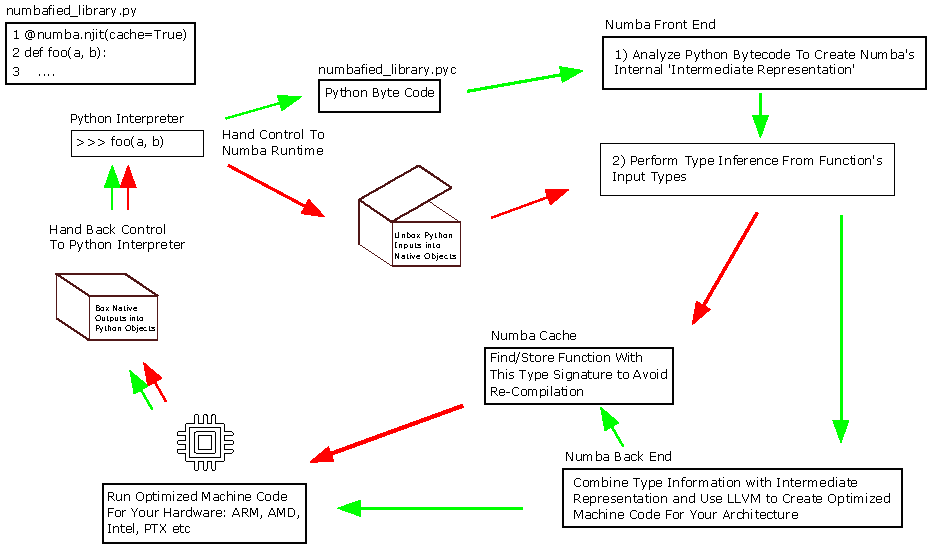
\includegraphics {figures/numba.pdf}}
    \caption{Simplified execution path when calling a Numba compiled function from the Python interpreter. The green path is only taken if the function hasn't been called before. The red path is taken if a compiled version with the correct type signature already exists in the Numba cache.}
    \label{fig:numba}
\end{figure*}

\lstinputlisting[float=t, caption={An example of using typed dictionaries in Numba.}\label{code:nested_function}]{nested_function.py}

\section{THE FAST MULTIPOLE METHOD}

The particle FMM is an approximation algorithm for $N$-body problems, in which $N$ source particles interact with $N$ target particles \cite{Greengard1987}. Consider the calculation of electrostatic potentials in 3D, which we use as our reference problem. A set of $N$ charged particles at positions $x_i$. The potential, $\phi_j$, at a given target particle at $x_j$ due to all other particles, excluding self interaction, can be written as.

\begin{equation}
    \phi_j = \sum_{i=1, i \neq j}^{N} \frac{q_i}{4 \pi| x_i-x_j |}
    \label{eq:laplace_kernel}
\end{equation}

where $\frac{1}{4 \pi| x_i-x_j|}$ is called the kernel, or the Green's function, and $q_i$ is the charge at $x_i$. The naive computation over all particles is $O(N^2)$, however the FMM compresses groups of interactions far away from a given particle using \textit{expansions}, reducing the overall complexity to $O(N)$. Expansions are ways of describing the charge contained within subregions of the octree, and can be truncated with to a desired accuracy, described by a parameter, $p$, called the expansion order. The value of $p$ is equal to the number of digits of precision of the final solution. Problems with this structure appear with such frequency in science and engineering that the FMM has been described as one of the ten most important algorithms of the twentieth century \cite{Cipra2000}.

The algorithm relies on a hierarchical octree data structure to discretize the problem domain in 3D (see fig. 1 \cite{Sundar2007}) and consists of eight operators: P2M, P2L, M2M, M2L, L2L, L2P, M2P and the `near field', applied \textit{once} to each applicable node over the course of two consecutive traversals of the octree (bottom-up and then top-down). An operator is read as `X to Y', where `P' stands for particle(s), `M' for \textit{multipole expansion} and `L' for \textit{local expansion}. The direct calculation of (\ref{eq:laplace_kernel}) is referred to as the P2P operator, and is used as a subroutine during the calculation of the other operators. The Kernel Independent FMM [KIFMM] \cite{Ying2004}, implemented by PyExaFMM and ExaFMM-T, is a re-formulation of the FMM with a structure that favours parallelization. Indeed all of the operators can be decomposed into matrix-vector products, or multithreaded implementations of (\ref{eq:laplace_kernel}), which are easy to optimize for modern hardware architectures, and fit well with Numba's programming framework. We defer to the FMM literature for a more detailed discussion on the mathematical significance of these operators \cite{Ying2004,Greengard1987}.

% Expansions are ways of describing the charge contained within subregions of the octree, and can be tuned to a given accuracy, described by a parameter called the expansion order, $p$. A multipole expansion represents the aggregation of charge located with a given node of the octree, where the expansion center is set to coincide with the box center. A multipole expansion can be translated into a local expansion centered on another node, inside of which it is valid. This is nothing other than the M2L operator, therefore the operators can be seen to be translations between expansion representations. Similarly, the expansion centers of local or multipole expansions can be shifted, which are the L2L and M2M operators respectively. The P2M/P2L operators forms a multipole/local expansion for a set of particles within a node. The M2P, L2P and P2P refer to directly evaluating the interaction in $O(N^2)$ between multipole/local expansion equivalent charges, or a set of source particles, at a set of target particles, respectively.

% In the KIFMM, multipole expansions are found by enclosing a node with an `equivalent surface' discretized with $n_e$ quadrature points, at each of which is placed an `equivalent charge'. A `check surface' discretized with $n_c$ quadrature points, is then used to enclose both the equivalent surface and the node, and a potential is calculated at the check surface using (\ref{eq:laplace_kernel}) directly with either the particles with the node (for P2M) or the equivalent charges of child nodes contained within the node (for M2M) as the source particles. Finally, a least-squares fit is used to match this calculated potential to that generated by the equivalent charges. Similar logic is used to calculate the M2L and L2L operators, with modified check and equivalent surfaces (see fig. 5 \cite{Ying2004}). The L2P, M2P, P2L and P2P operators all involve using (\ref{eq:laplace_kernel}) for direct evaluations, rather than a least-squares fit.

\section{COMPUTATIONAL STRUCTURE OF FMM OPERATORS}

The computational complexities of KIFMM operators are defined by a user specified $n_{crit}$, which is the maximum allowed number of particles in a leaf node, $n_e$ and $n_c$ which are the numbers of quadrature points on the \textit{check} and \textit{equivalent} surfaces respectively (see sec. 3 \cite{Ying2004}). The parameters $n_e$ and $n_c$ are quadratically related to the expansion order, i.e. $p \sim n_e^2$. Typical values for $n_{crit}$ used are $\sim 100$. Notice the depth of the octree is defined $n_{crit}$, and hence by the particle distribution.

The near field, P2M, P2L, M2P, and L2P only operate on leaf nodes. The M2L operates during the top-down traversal from level two downwards, operating on all nodes at a given level during each step. The M2M is applied to each node during the bottom-up traversal, and the L2L is applied to each node during the top-down traversal.

All operators, except the M2L M2M and L2L, rely on the P2P. The inputs for the P2P are vectors for the source and target positions, and the source charges or expansion coefficients (which approximate charges). The output is a vector of potentials.

The inputs to the M2L, M2P, P2L and near field operators are defined by `interaction lists', called the V, W, X and U lists respectively. These interaction lists define the nodes a target node interacts with when an operator is applied to it. We can restrict the size of these interaction lists by demanding that neighboring nodes at the leaf level are at most twice as large as each other \cite{Sundar2007}. Using this `balance condition', the V, X, W and U lists contains at most 189, 19, 148 and 60 nodes in three dimensions, respectively.

The near field operator applies the P2P between the charges contained in the target and the source particles of nodes in its U list, in $O(60 \cdot n_{crit}^2)$. The M2P applies the P2P between multipole expansion coefficients of source nodes in the target's W list and the charges it contains in $O(148 \cdot n_e \cdot n_{crit})$. Similarly, the L2P applies the P2P between a target's own local expansion coefficients and the charges it contains in $O(n_e \cdot n_{crit})$.

The P2L, P2M and M2L involve creating local and multipole expansions, and rely on a matrix vector product related to the number of source nodes being compressed, which for the P2L and M2L are defined by the size of the target node's interaction lists. These matrix vector products have complexities of the form $O(k \cdot n_e^2)$ where $k = |X| = 19$ for the P2L, $k = |V| = 189$ for the M2L, and $k = 1$ for the P2M. Additionally, the P2L and P2M have to calculate `check potentials' (see sec. 3 \cite{Ying2004}) which require $O(19 \cdot n_{crit} \cdot n_c)$ and $O(n_{crit} \cdot n_c)$ calculations respectively. The M2M and L2L operators both involve translating expansions between nodes their eight children, and rely on a matrix vector product of $O(n_e^2)$.

The structure of the FMM's operators expose natural parallelism. The P2P is embarrassingly parallel over each target. As are the M2L, M2P, P2L and near field operators over their interaction lists. The near field, L2P, M2P, P2L and P2M operators are also embarrassingly parallel over the leaf nodes, as is the M2L over the nodes at a given level, and the M2M and L2L over sibling nodes which share a parent.

\section{MULTITHREADING IN NUMBA}

One of the main selling points of Numba is that it allows multithreading via a simple parallel for loop syntax (listing (\ref{code:parallel_multithreading})) reminiscent of OpenMP's syntax. Numba can compile parallel code using either OpenMP, or Intel TBB as the backend software actually creating the multithreaded code. We choose OpenMP for PyExaFMM, as TBB is more suited for parallel workloads that may be irregular in size.

- Thread oversubscription issues and their origin and how to avoid this in Numba. Comment on the quality of this solution - the py multithreading papers from intel group have good information and experiments regarding this.

- how kernels are multithreaded bearing in mind issues raise in Numba section, and data oriented design section.

- Optimal design of multithreading approach relies on the actual constraints of the kernel in question, will need to get into specifics here of how each kernel was approached.

- metric for portion of code that is run on single vs multiple threads, can actually time this at least roughly.

M2M
- serial. cannot parallelize over leaves, there are parallel writes to parent multipole expansion from siblings. Parallelizing over sibling leaves is hard due to linear representation of tree - have to perform expensive neighbours searches to find siblings to perform group by. equivalent charge = $O(8^l \cdot n_e \cdot n_c)$ at a given level $l$.

\lstinputlisting[float=t, caption={An example of parallel multithreading.}\label{code:parallel_multithreading}]{parallel_multithreading.py}

\section{DATA ORIENTED DESIGN FOR NUMBA}

- what is data oriented design? Why is it necessary? Why does Numba demand this?

- we implement it in three ways: (1) the simplicity of our containers, few abstractions (2) Our thin API in Python, shelving off most functionality to numba (3)

- long nested operator functions

- multipole and local expansions of whole tree stored as long 1D arrays

- API designed

- Minimize the impact of running code in the interpreter.

% Larger figure
\begin{figure*}
    \centerline{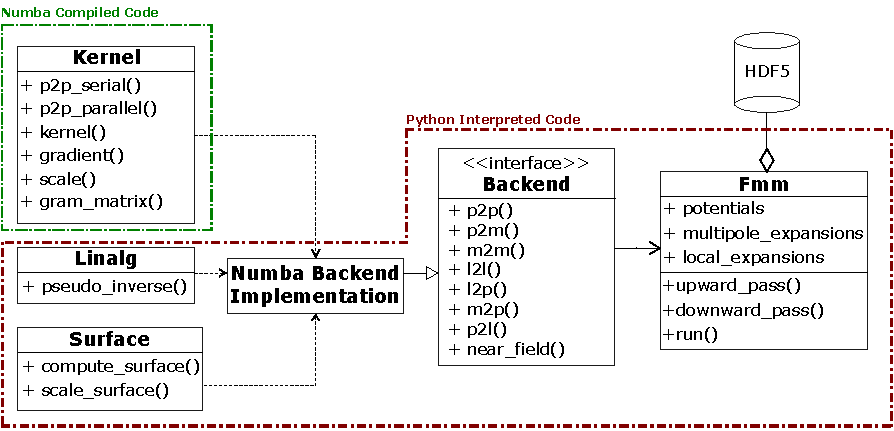
\includegraphics {figures/software.pdf}}
    \caption{Simplified UML model of all PyExaFMM components. Trees and operators are precomputed and stored in the HDF5 database. The `Fmm' object which acts as the user interface, all other components are modules consisting of methods on operating on arrays.}
    \label{fig:design}
\end{figure*}

\section{DIFFERENCES WITH EXAFMM-T}

- tree design is linear.

- things this makes hard - neighbor searches.

- things it makes easy - easy interoperability with numba
A strict like-for-like comparison between the two implementations isn't possible. The softwares take different approaches to the implementation of some of their operations and data structures. However, as the differences in the design of PyExaFMM are heavily influenced by Numba and Python, it remains useful as an illustration of what can be achieved with Python in comparison to a compiled language to solve the same problem.

- Main differences are tree design, and the replacement of FFT with rSVD.

- A short note on the decision for M2l via SVD, and the expected impact on performance - condense discussion from MSc thesis section 2.4 pg 28

\section{BENCHMARKS}

- contrast multithreading impact for each kernel

- boxing cost for each kernel

- compare and contrast pyexafmm vs exafmm for a given accuracy, try and find optimum compression parameter.(?)

\section{CONCLUSION}

We've shown how to use Numba to create a performant application for an algorithm with a complex data structure. We've shown where Numba can constrain software design, and that developers must be careful in order to experience a performance benefit. Achieving performance for complex implementations requires more software knowledge than non-software specialists can be expected to have, and Numba can be seen to have its own learning curve. Despite this, Numba is a remarkable tool, allowing the development of fast, heterogenous, cross-platform numerical applications, all from Python. Projects which favour hackability or have a small number of performance bottlenecks would benefit the most from a Numba implementation.

\section{ACKNOWLEDGMENT}

SK is sported by EPSRC Studentship 2417009.

\bibliography{pyexafmm}

\bibliographystyle{ieeetr}

\begin{IEEEbiography}{Srinath Kailasa}{\,}is a PhD student in Mathematics at University College London. Contact him at srinath.kailasa.18@ucl.ac.uk.
\end{IEEEbiography}

\begin{IEEEbiography}{Tingyu Wang}{\,}is a PhD student in Mechanical Engineering at the George Washington University. Contact him at twang66@email.gwu.edu.
\end{IEEEbiography}

\begin{IEEEbiography}{Lorena. A. Barba}{\,}is a Professor of Mechanical and Aerospace Engineering at the George Washington University.  Contact her at labarba@email.gwu.edu.
\end{IEEEbiography}

\begin{IEEEbiography}{Timo Betcke}{\,}is Professor of Computational Mathematics at University College London. Contact him at t.betcke@ucl.ac.uk.
\end{IEEEbiography}

\end{document}

